\documentclass[xcolor=dvipsnames]{beamer}


\usetheme[
          showdate=true,                     % show the date on the title page
          alternativetitlepage=true,         % Use the fancy title page.
          titlepagelogo=general_figures/shell,              % Logo for the fir\
st page.
          ]{UMD}

%\usetheme{Rochester}

%\usepackage{beamerthemesplit}
\usepackage{xmpmulti}

\usepackage{booktabs}
\usepackage{graphicx,float,wrapfig, bbm}
\usepackage{tabularx}
\usepackage{amsfonts, bbold, comment}
\usepackage{mdwlist}
\usepackage{tikz}
\usepackage{subfigure}
\usepackage{colortbl}
\usepackage[normalem]{ulem}

\usepackage{multirow}

\usetikzlibrary{shapes.geometric}
\definecolor{xred}{HTML}{DB4437}
\definecolor{xyellow}{HTML}{F4B400}
\definecolor{xgreen}{HTML}{0F9D58}

\newcommand*{\tcircle}[1]{\tikz[anchor=base,baseline=-2.5pt] \node[circle,fill=#1,scale=0.9] (X) {};}
\newcommand*{\tsquare}[1]{\tikz[anchor=base,baseline=-2.5pt] \node[fill=#1,scale=1.2] (X) {};}
\newcommand*{\tdiamond}[1]{\tikz[anchor=base,baseline=-2.5pt] \node[diamond,fill=#1,scale=0.7] (X) {};}
\newcommand*{\ttriangle}[1]{\tikz[anchor=base,baseline=-1.5pt] \node[regular polygon,regular polygon sides=3,fill=#1,scale=0.6] (X) {};}



\newcommand{\fsi}[2]{
\begin{frame}[plain]
\vspace*{-1pt}
\makebox[\linewidth]{\includegraphics[width=\paperwidth]{#1}}
\begin{center}
#2
\end{center}
\end{frame}
}

\newcommand{\abr}[1]{\textsc{#1} }
\newcommand{\pos}[1]{{\texttt{#1}}}
\newcommand{\e}[2]{\mathbb{E}_{#1}\left[ #2 \right] }
\newcommand{\ind}[1]{\mathbb{I}\left[ #1 \right] }
\newcommand{\ex}[1]{\mbox{exp}\left\{ #1\right\} }
\newcommand{\g}{\, | \,}
\newcommand{\citename}[1]{#1 }

\newcommand{\gfxd}[2]{
\begin{center}
	\includegraphics[width=#2\linewidth]{diplomacy/#1}
\end{center}
}

\newcommand{\gfxq}[2]{
\begin{center}
	\includegraphics[width=#2\linewidth]{qb/#1}
\end{center}
}



%\usecolortheme{ucdblack}
\title[Trick me if you can]{Engaging Hobbyist Communities to Decieve Machines and Each Other}
\author{ Jordan Boyd-Graber et al.}
\date{2019}

\institute[Maryland] % (optional, but mostly needed)
{University of Maryland}

\begin{document}

\frame{
\titlepage
\tiny
}

\fsi{qb/turing}{Turing Test: Definition of AI (Image from Wall Street
  International)}

\begin{frame}{Overview}

\begin{itemize}
  \item Computers need to learn how to deal with tricky text
  \item How do we get it?
  \item Creativity in crowdsourcing is hard to motivate
  \item Getting professional trivia writers to trick machines
  \item Getting humans to lie to each other
\end{itemize}

\end{frame}

\fsi{qb/jeopardy}{IBM Watson: QA Solved!}

\fsi{qb/human_reading}{SQuAD: Ignore Knowledge}


\begin{frame}
	\frametitle{Disproving this claim\dots}
	\begin{columns}

	\column{.5\linewidth}
	\begin{itemize}
		\item Game called ``quiz bowl''
		\item Two teams play each other
		\begin{itemize}
			\item Moderator reads a question
			\item When a team knows the answer, they signal (``buzz'' in)
			\item If right, they get points; otherwise, rest of the question is read to the other team
		\end{itemize}
	      \item Hundreds of teams in the US alone
                \only<2->{A rich, active community}
                \only<3>{\item Example \dots}
	\end{itemize}

	\column{.5\linewidth}
	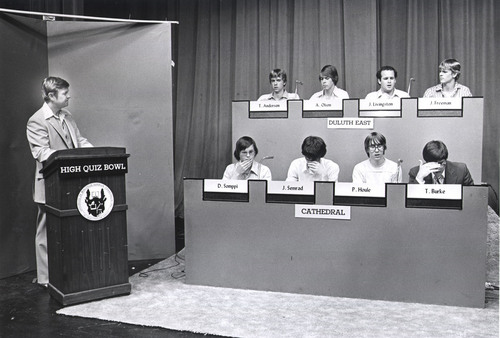
\includegraphics{qb/quizbowl}

	\end{columns}

\end{frame}


\begin{frame}[t]
	\frametitle{Sample Question}

        The Swiss-Italian architect Pietro Antonio Solari
        \only<2->{built several fortified towers in this city, which
          often vied for power with its northern rival Tver. A ruler
          of this city prevailed in the} \only<3->{Great Stand on the
          Ugra River. A prince from this city was nicknamed for
          winning a battle on the} \only<4->{Don river. Partly because
          a ruler of this city married} \only<5->{Sophia Palaiologina,
          the niece of the last Byzantine Emperor, this city styled
          itself the} \only<6->{``Third Rome'' after the fall of
          Constantinople. Another prince of this city stopped paying
          tribute to the} \only<7->{Mongols in 1476, ending the
          ``Tatar yoke.''} \only<8->{The Grand Duchy headquartered in
          this city came to an end in 1547 with the ascension of}
        \only<9->{ Ivan IV, who made it his capital. For 10 points,
          name this city where Ivan III renovated the
          Kremlin,} \only<10->{the capital of Russia.}\\
        \vspace{.5cm} \only<11->{ {\bf Moscow} (Moskva / Muscovy)}

\end{frame}


\begin{frame}
	\frametitle{Question Structure Enables Compeition}

	\begin{columns}
		\column{.5\linewidth}

		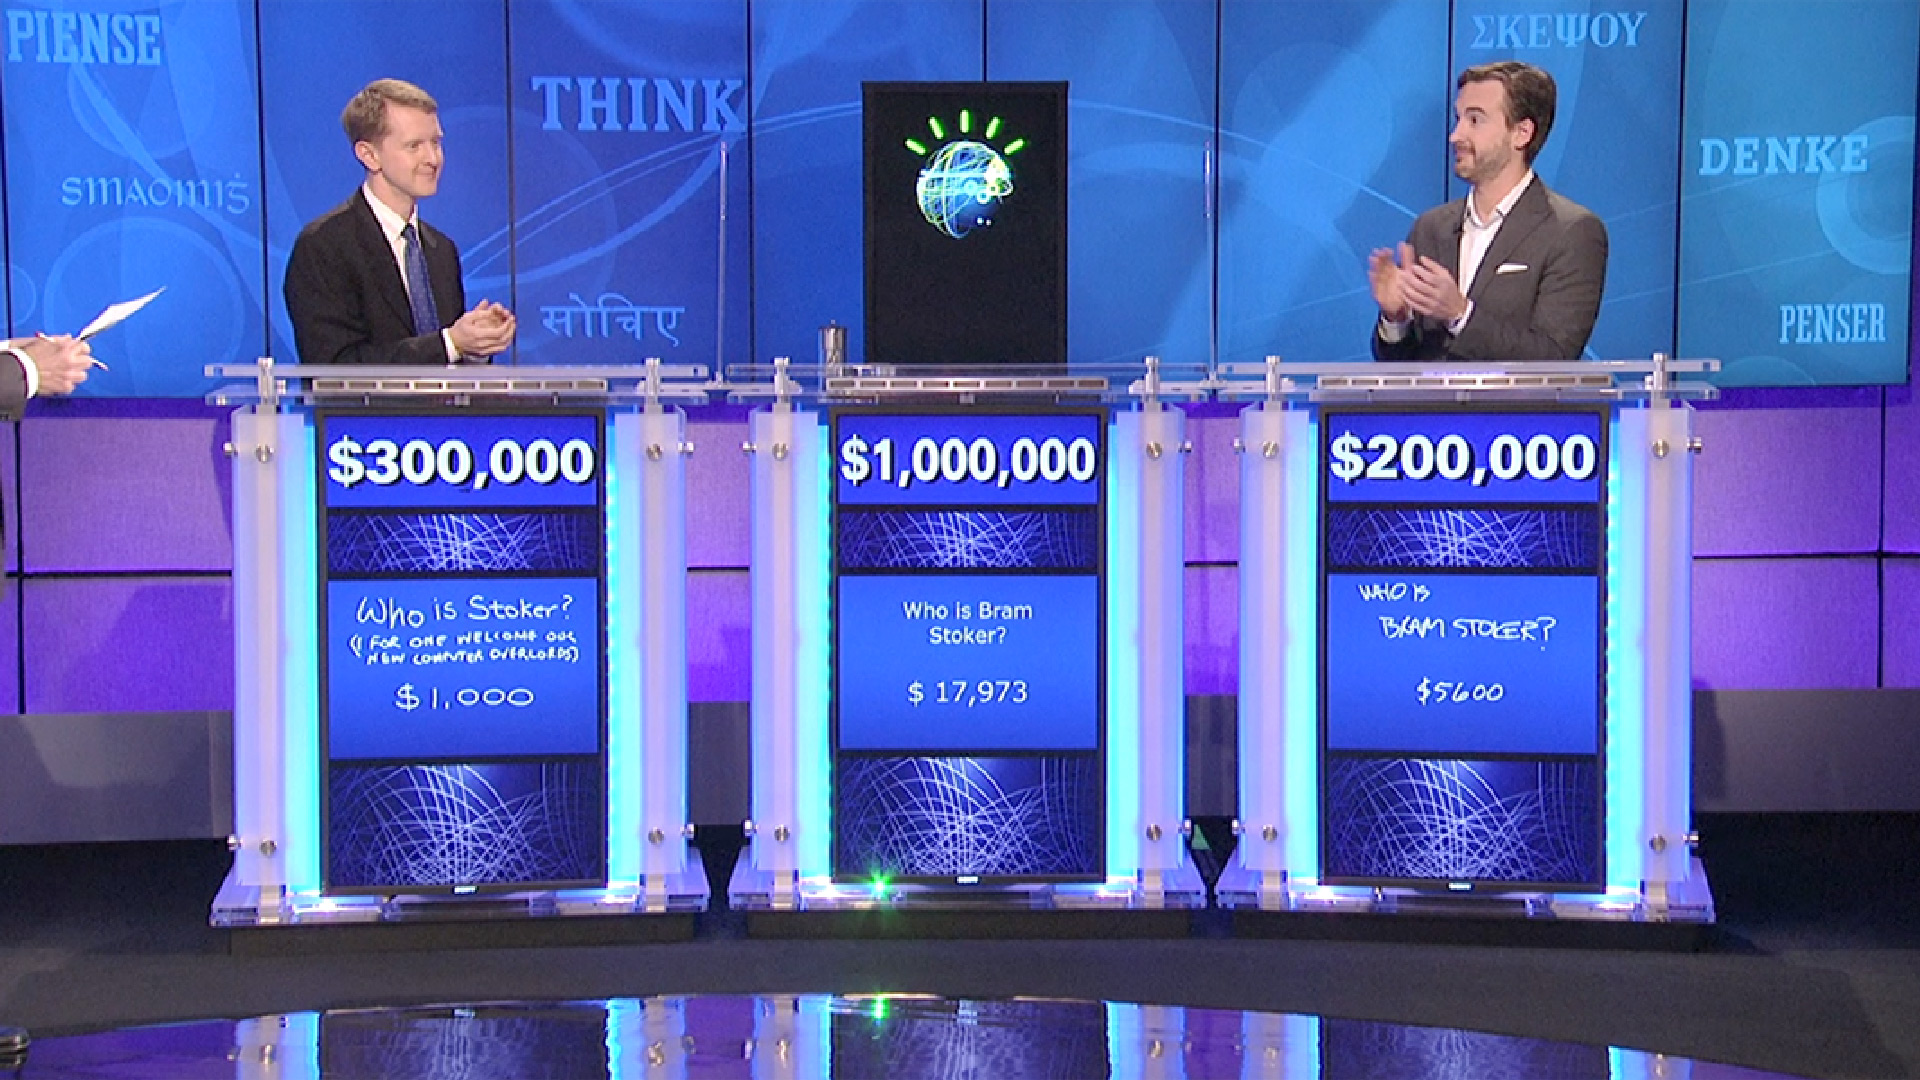
\includegraphics[width=1.0\linewidth]{qb/jeopardy}


		\column{.5\linewidth}
		\begin{itemize}
                        \item Watson must decide to answer {\bf once}, after
                          complete question
                        \item Quiz Bowl: decide after each word
                        \item Obscure clues at start, easy at end
                        \item ``Gold standard'' in trivia community
		\end{itemize}

	\end{columns}

\end{frame}


\begin{frame}{}

  \begin{columns}
    \column{.5\linewidth}
        
\includegraphics[width=0.7\linewidth]{general_figures/hehe}
    \column{.5\linewidth}
        \begin{block}{{\bf
              \href{http://cs.colorado.edu/~jbg//docs/qb_emnlp_2012.pdf}{Besting
                the Quiz Master: Crowdsourcing Incremental
                Classification Games}}}

          {\bf Jordan Boyd-Graber}, He He, and Hal {Daum\'{e} III}. \emph{Empirical Methods in Natural Language Processing}, 2012
        \end{block}
  \end{columns}
\end{frame}


\begin{frame}
\frametitle{Interface}

\begin{columns}

	\column{0.5\linewidth}

	\begin{center}
		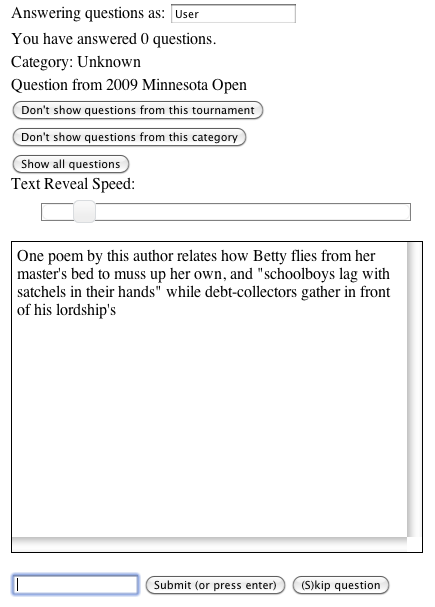
\includegraphics[width=0.8\linewidth]{qb/screenshot}
	\end{center}

	\column{0.5\linewidth}


	\only<2>{
	\begin{itemize}
		\item 7000 questions: first day
		\item 43000 questions: two weeks
		\item 461 unique users
                \item Imitated \dots
	\end{itemize}
        \gfxq{protobowl}{.8}
	}



\end{columns}
\end{frame}


\begin{frame}{Computers are Good at Memorizing}

  \begin{center}
  \href{https://www.youtube.com/watch?v=MzM1oNsm8MQ&feature=youtu.be&t=136&autoplay=1}{Poems, TV Shows, Artwork}
  \end{center}
    \gfxq{hsnct_2017}{1.0}
   
\end{frame}



\begin{frame}{Can we improve QA systems?}

\begin{columns}
  \column{.6\linewidth}
     \gfxq{trick/pyramid}{.9}
     \column{.4\linewidth}
     \begin{itemize}
       \item Questions should be pyramidal
       \item But for whom?
         \begin{itemize}
           \item Quotes
           \item Reusing clues
         \end{itemize}
         \item Adversarial writing
         \item Improve questions
     \end{itemize}
\end{columns}
\end{frame}



\fsi{general_figures/blackbox}{}
  
\begin{frame}{What do we mean by ``adversarial''?}

  \gfxq{trick/flow_chart_horizontal_label}{1.0}

  \begin{itemize}
    \item Round 1: Only IR interpretations
    \item Round 2: IR and RNN (influence functions) interpretations
      \pause
    \item Another reason we need to have good explanations of QA
  \end{itemize}

\end{frame}

\begin{frame}{But why?}

  \begin{itemize}
  \item Fair comparison
  \item Improve computer question answering
  \item Understand where computers struggle
    \item Explain how computers answer questions better
  \end{itemize}

\end{frame}


\fsi{qb/trick/brahms_0}{\href{http://write.qanta.org}{http://write.qanta.org}}
\fsi{qb/trick/brahms_1}{}
\fsi{qb/trick/brahms_2}{}
\fsi{qb/trick/brahms_3}{}
\fsi{qb/trick/brahms_4}{}
\fsi{qb/trick/brahms_5}{}


\fsi{qb/trick/round_one}{Round 1: Only IR-based QA system}
\fsi{qb/trick/round_two}{Round 2: RNN-based QA system}


\begin{frame}{Competition}

  \gfxq{trick/pace}{.8}

\begin{itemize}
  \item December 15: Seven top human teams, fourteen computer teams
  \item Top four teams from each ``division'' faced off against each
    other
    \pause
  \item All computer teams lost to human teams
    \pause
  \item But two games were really close; strongest system was based on BERT
  \item YouTube video series! \dots
\end{itemize}

\end{frame}

% Hard but not really a good question: F3 Q24

\begin{frame}{Impossible Until the End}
\alert<3>{Ritchie Watson commended this play's historical accuracy for
  getting the price for a dozen eggs right---ten cents---to defend
  against Elizabeth Hardwick’s contention that it was a sentimental
  history.} \alert<4>{At the end of this play, a man wonders why a wheelchair is
at the top of a staircase, and} \alert<5>{Alexandra announces that she is leaving
her mother. Leo is pressured into stealing a set of valuable railroad
bonds in this drama. In this play, which takes its title from the Song
of Solomon,} Regina Hubbard schemes  \tdiamond{xgreen}
\tcircle{xgreen} to obtain a majority share in a cotton mill. For 10
points,  \tsquare{xgreen}  \ttriangle{xgreen} name this play by
Lillian Hellman. \\

\pause

\textbf{Answer}: The\ Little\ Foxes\\

\only<3>{Academic literature}
\only<4>{Vague plot summary}
\only<5>{Avoid last names}

\end{frame}

% Tricky and hard: F3 Question 25

\begin{frame}{Tricky and impossible for current systems}
In Our Town, a character  \ttriangle{xred} with this given name explains Grover’s Corners’ place in the universe. In The Crucible, a character  \tcircle{xred} with this first name contends that the girls’ actions are part of their “silly seasons” and is the wife of Francis Nurse. A novel with this name, which conducts hidden messages to Rommel in The English Patient, is titled for a character who is killed in a boating accident at Manderley. For 10 points, give this name of a Daphne du Maurier  \tdiamond{xyellow}  \tsquare{xgreen} gothic novel which is also the first name of Miss Sharp, the protagonist of William Thackeray's Vanity Fair. \tcircle{gray}  \ttriangle{gray}


\ttriangle{xred} Thornton Wilder
\tcircle{xred} Richard
\tcircle{gray} Richard
\ttriangle{gray} Thornton Wilder \\
\textbf{Answer}: Rebecca\\
\end{frame}

% Tricky and hard: F3 Question 29

\begin{frame}{Close, but \dots}
An army that took its name from this geographical feature had a
British doctor, James Paroissien, as its Surgeon General, and recent
scholarship by Peter Blanchard revealed its use of slaves. That army
crossed this geographical feature according  \ttriangle{xred} to
Thomas Maitland’s  \tcircle{xred} plans at Uspallata and Los
Patos. Spanish forces under Rafael Maroto were defeated in the
foothills of these mountains by an army led by José de San Martín and
Bernardo O'Higgins.  \tsquare{xred} For 10 points, name this mountain
range of South America that played a role  \ttriangle{xyellow} in the
independence of Chile. \tdiamond{gray}  \tcircle{gray}  \tsquare{gray}

\ttriangle{xred} Angel Falls
\tcircle{xred} Mountain
\tsquare{xred} Battle of Chacabuco
\tdiamond{gray} Battle of Chacabuco
\tcircle{gray} Mountain
\tsquare{gray} Battle of Chacabuco \\
\pause
\textbf{Answer}: Andes\\

\end{frame}

% Showing strength of QB format: Packet F3 Question 30

\begin{frame}{Showing the strength of quiz bowl format}
A painting by this artist  \tsquare{xred} presents a tree as a cupboard with two doors, behind which are a white sphere and a miniature lighted house. A series of three paintings by this man shows a daytime sky with cumulus clouds above a dark house illuminated by a lamppost. This artist of Blood Will Tell and The Empire of Lights depicted a clock set to 12:43  \tcircle{xgreen} as a locomotive speeds out of a fireplace and a man in  \tsquare{xyellow} a bowler hat with an  \ttriangle{xgreen} apple in front of his face. For 10 points, name this Belgian surrealist painter  \tdiamond{xgreen} of the Son of Man and Time Transfixed.

\tsquare{xred} Argon \\
\pause
\textbf{Answer}: René\ Magritte\\
\end{frame}




% Why it's a good learning framework: Packet F3 Question 31




\begin{frame}{My favorite example}
\begin{center}
\only<3>{The narrator in Cogwheels by} \alert<3>{this author opens \emph{Crime and Punishment}} \only<3>{to find it be The Brothers Karamazov}
\end{center}

\only<2>{\gfxq{dostoyevski}{.3}}
\only<3>{\gfxq{akutagawa}{.3}}

\end{frame}


\begin{frame}{Future \dots}

  \begin{itemize}
    \item Computers dominate on ``normal'' questions
    \item Not so much on adversarial questions
    \item Stronger QA systems 
      \begin{itemize}
        \item Need more thought on how to explain
        \item Expose QA system to more users
        \item Increase the breadth of resources
        \item Multilingual
      \end{itemize}
  \end{itemize}

\end{frame}




\begin{frame}{Find out More!}

		\begin{itemize}
			\item Code: \url{http://github.com/Pinafore/qb}
                        \item Shared Task \url{http://trickme.qanta.org}
		\end{itemize}

    \end{frame}

\begin{frame}{}

  \begin{columns}
    \column{.5\linewidth}
        
\includegraphics[width=0.7\linewidth]{general_figures/vlad}
    \column{.5\linewidth}
        \begin{block}{{\bf
              \href{http://cs.colorado.edu/~jbg//docs/2015_acl_diplomacy.pdf}{Linguistic Harbingers of Betrayal: A Case Study on an Online Strategy Game}}}

          Vlad Niculae, Srijan Kumar, Jordan Boyd-Graber, and Cristian
          Danescu-Niculescu-Mizil. \emph{Association for Computational Linguistics}, 2015
        \end{block}

  \end{columns}
\end{frame}


\begin{frame}{Man's Dishonesty to Man}

  \begin{itemize}
  \item Tricking computers helps computers learn
  \item But humans tricking humans is a bigger problem
    \begin{itemize}
    \item Fraud
    \item Phishing
      \item Political framing / spin
      \end{itemize}
    \item Difficult to apply standard classification
      \pause
    \item Before, we turned to a vibrant community to generate
      inventive text\dots
  \end{itemize}

\end{frame}

\fsi{diplomacy/tournament}{A Community of Liars}

\begin{frame}[plain]
\vspace*{-1pt}
\only<1>{\makebox[\linewidth]{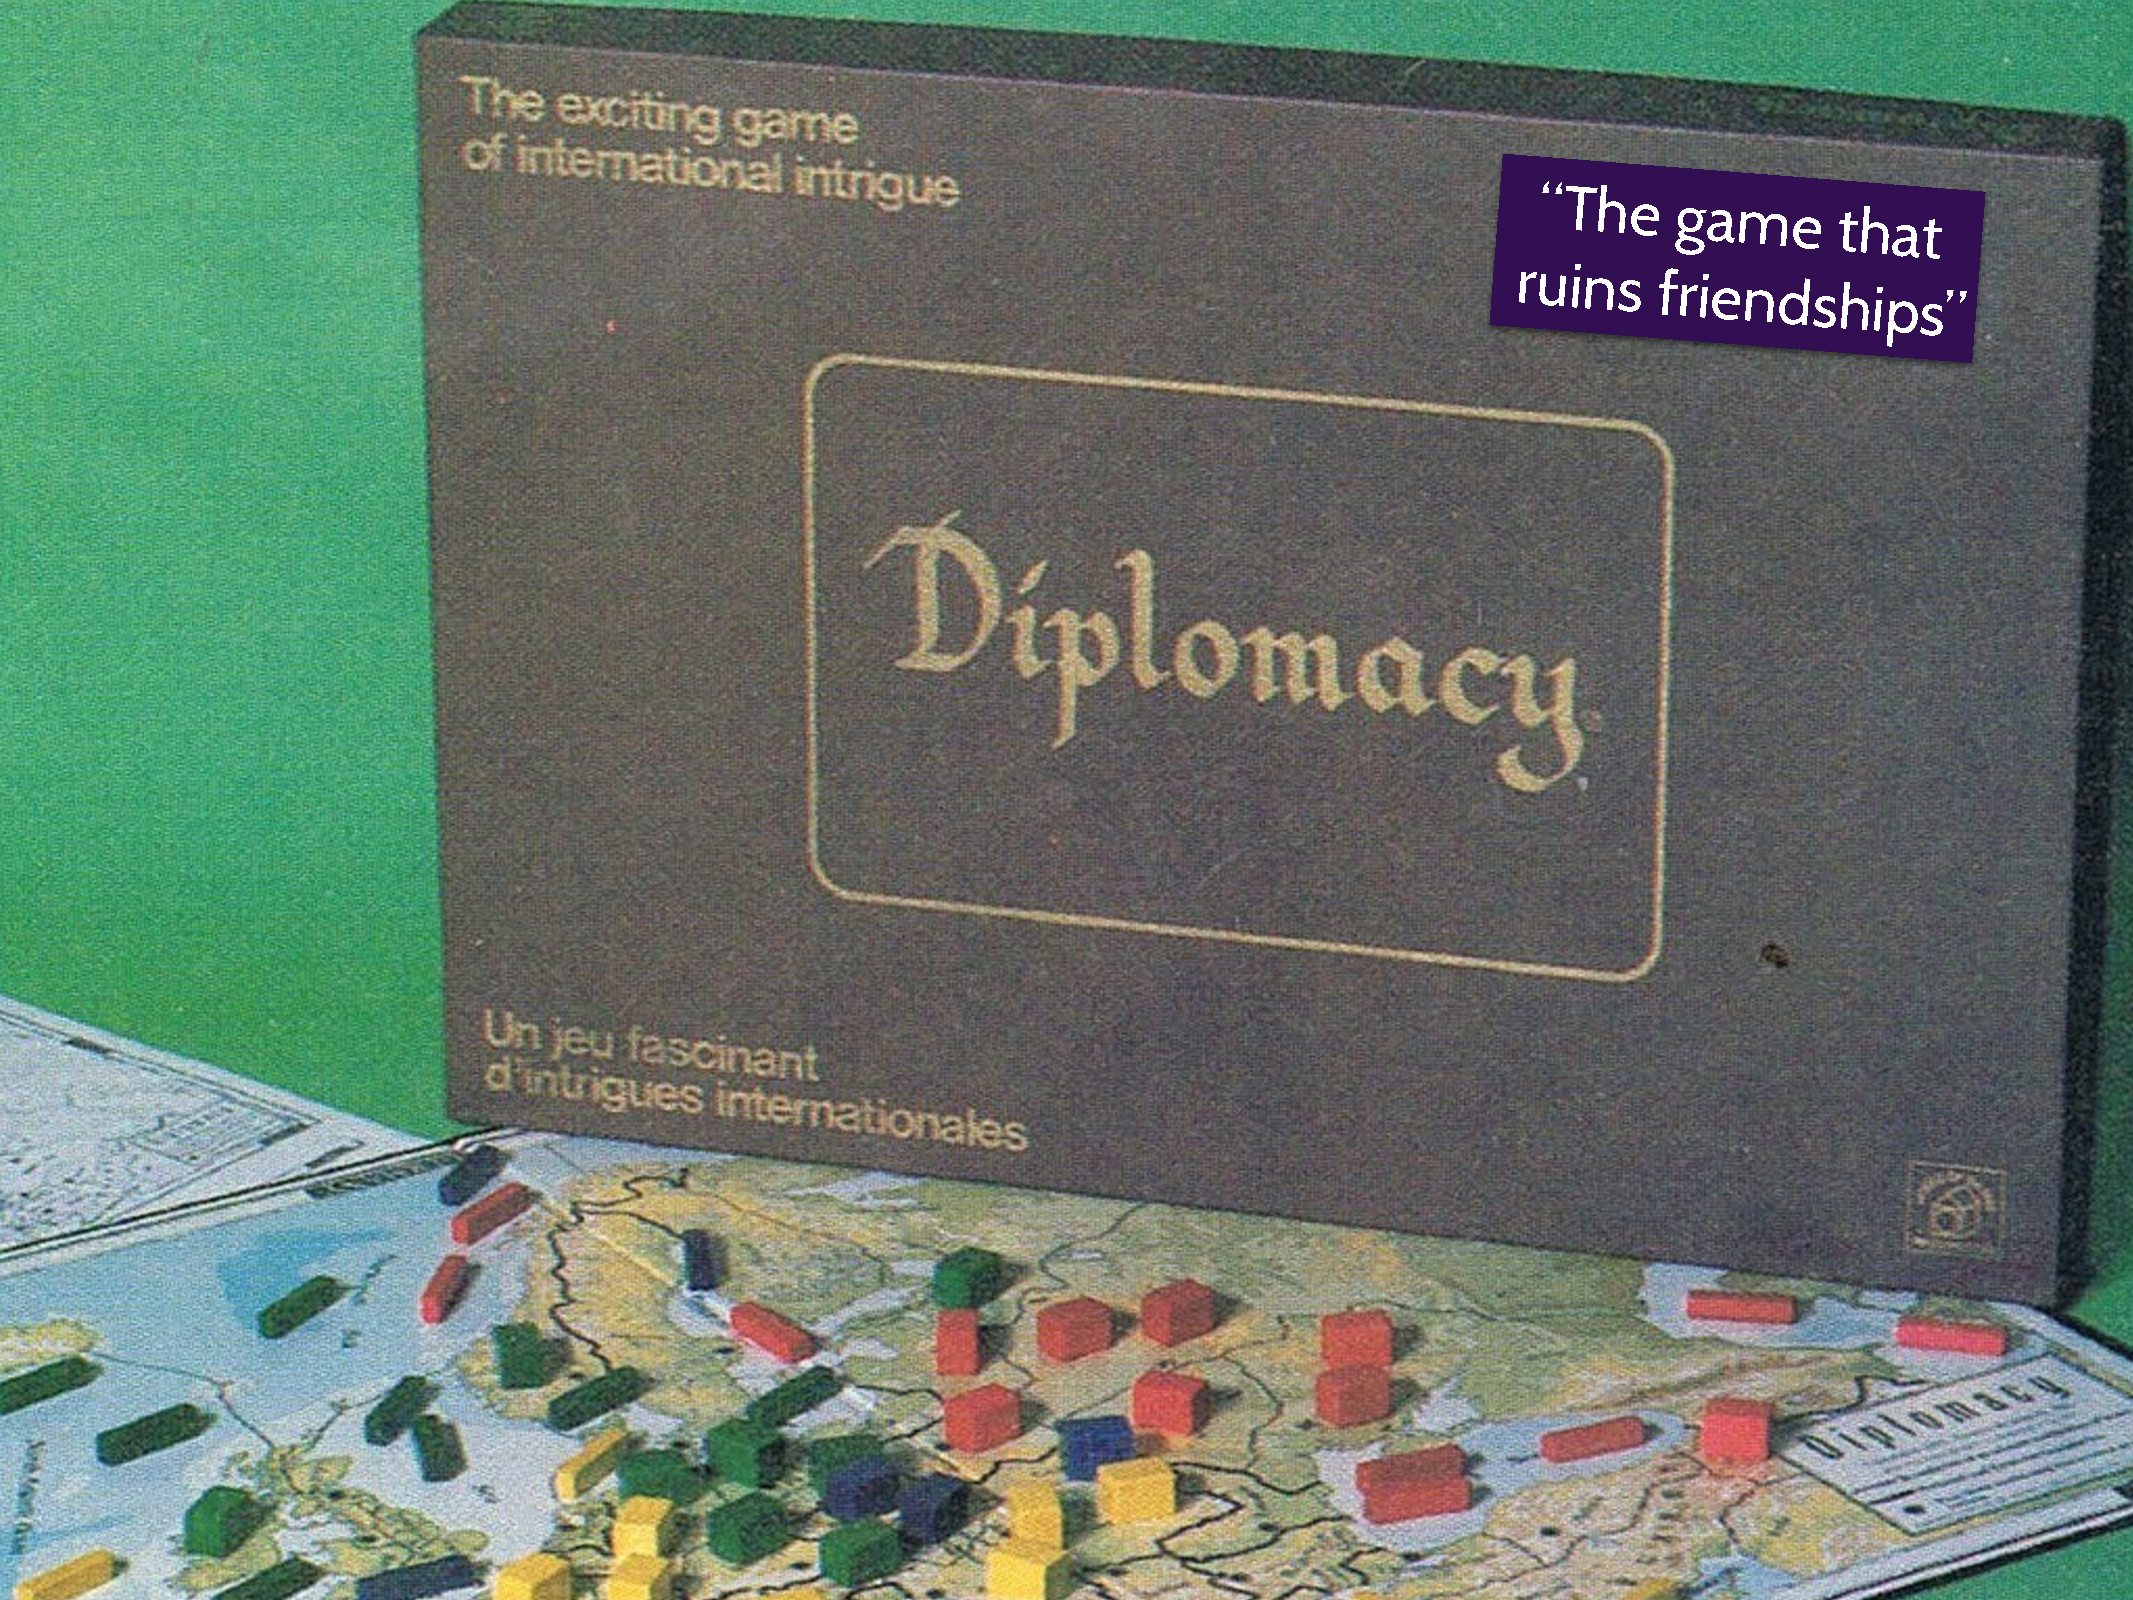
\includegraphics[page=1,width=\paperwidth]{diplomacy/betrayal-slides}}}
\only<2>{\makebox[\linewidth]{\includegraphics[page=2,width=\paperwidth]{diplomacy/betrayal-slides}}}
\only<3>{\makebox[\linewidth]{\includegraphics[page=3,width=\paperwidth]{diplomacy/betrayal-slides}}}
\only<4>{\makebox[\linewidth]{\includegraphics[page=4,width=\paperwidth]{diplomacy/betrayal-slides}}}
\only<5>{\makebox[\linewidth]{\includegraphics[page=5,width=\paperwidth]{diplomacy/betrayal-slides}}}
\only<6>{\makebox[\linewidth]{\includegraphics[page=6,width=\paperwidth]{diplomacy/betrayal-slides}}}
\only<7>{\makebox[\linewidth]{\includegraphics[page=7,width=\paperwidth]{diplomacy/betrayal-slides}}}
\only<8>{\makebox[\linewidth]{\includegraphics[page=8,width=\paperwidth]{diplomacy/betrayal-slides}}}
\only<9>{\makebox[\linewidth]{\includegraphics[page=9,width=\paperwidth]{diplomacy/betrayal-slides}}}
\only<10>{\makebox[\linewidth]{\includegraphics[page=10,width=\paperwidth]{diplomacy/betrayal-slides}}}
\only<11>{\makebox[\linewidth]{\includegraphics[page=11,width=\paperwidth]{diplomacy/betrayal-slides}}}
\only<12>{\makebox[\linewidth]{\includegraphics[page=12,width=\paperwidth]{diplomacy/betrayal-slides}}}
\only<13>{\makebox[\linewidth]{\includegraphics[page=13,width=\paperwidth]{diplomacy/betrayal-slides}}}
\only<14>{\makebox[\linewidth]{\includegraphics[page=14,width=\paperwidth]{diplomacy/betrayal-slides}}}
\only<15>{\makebox[\linewidth]{\includegraphics[page=15,width=\paperwidth]{diplomacy/betrayal-slides}}}
\only<16>{\makebox[\linewidth]{\includegraphics[page=16,width=\paperwidth]{diplomacy/betrayal-slides}}}
\only<17>{\makebox[\linewidth]{\includegraphics[page=17,width=\paperwidth]{diplomacy/betrayal-slides}}}
\only<18>{\makebox[\linewidth]{\includegraphics[page=18,width=\paperwidth]{diplomacy/betrayal-slides}}}
\only<19>{\makebox[\linewidth]{\includegraphics[page=19,width=\paperwidth]{diplomacy/betrayal-slides}}}
\only<20>{\makebox[\linewidth]{\includegraphics[page=20,width=\paperwidth]{diplomacy/betrayal-slides}}}
\only<21>{\makebox[\linewidth]{\includegraphics[page=21,width=\paperwidth]{diplomacy/betrayal-slides}}}
\end{frame}

\begin{frame}[plain]
\vspace*{-1pt}
\only<1>{\makebox[\linewidth]{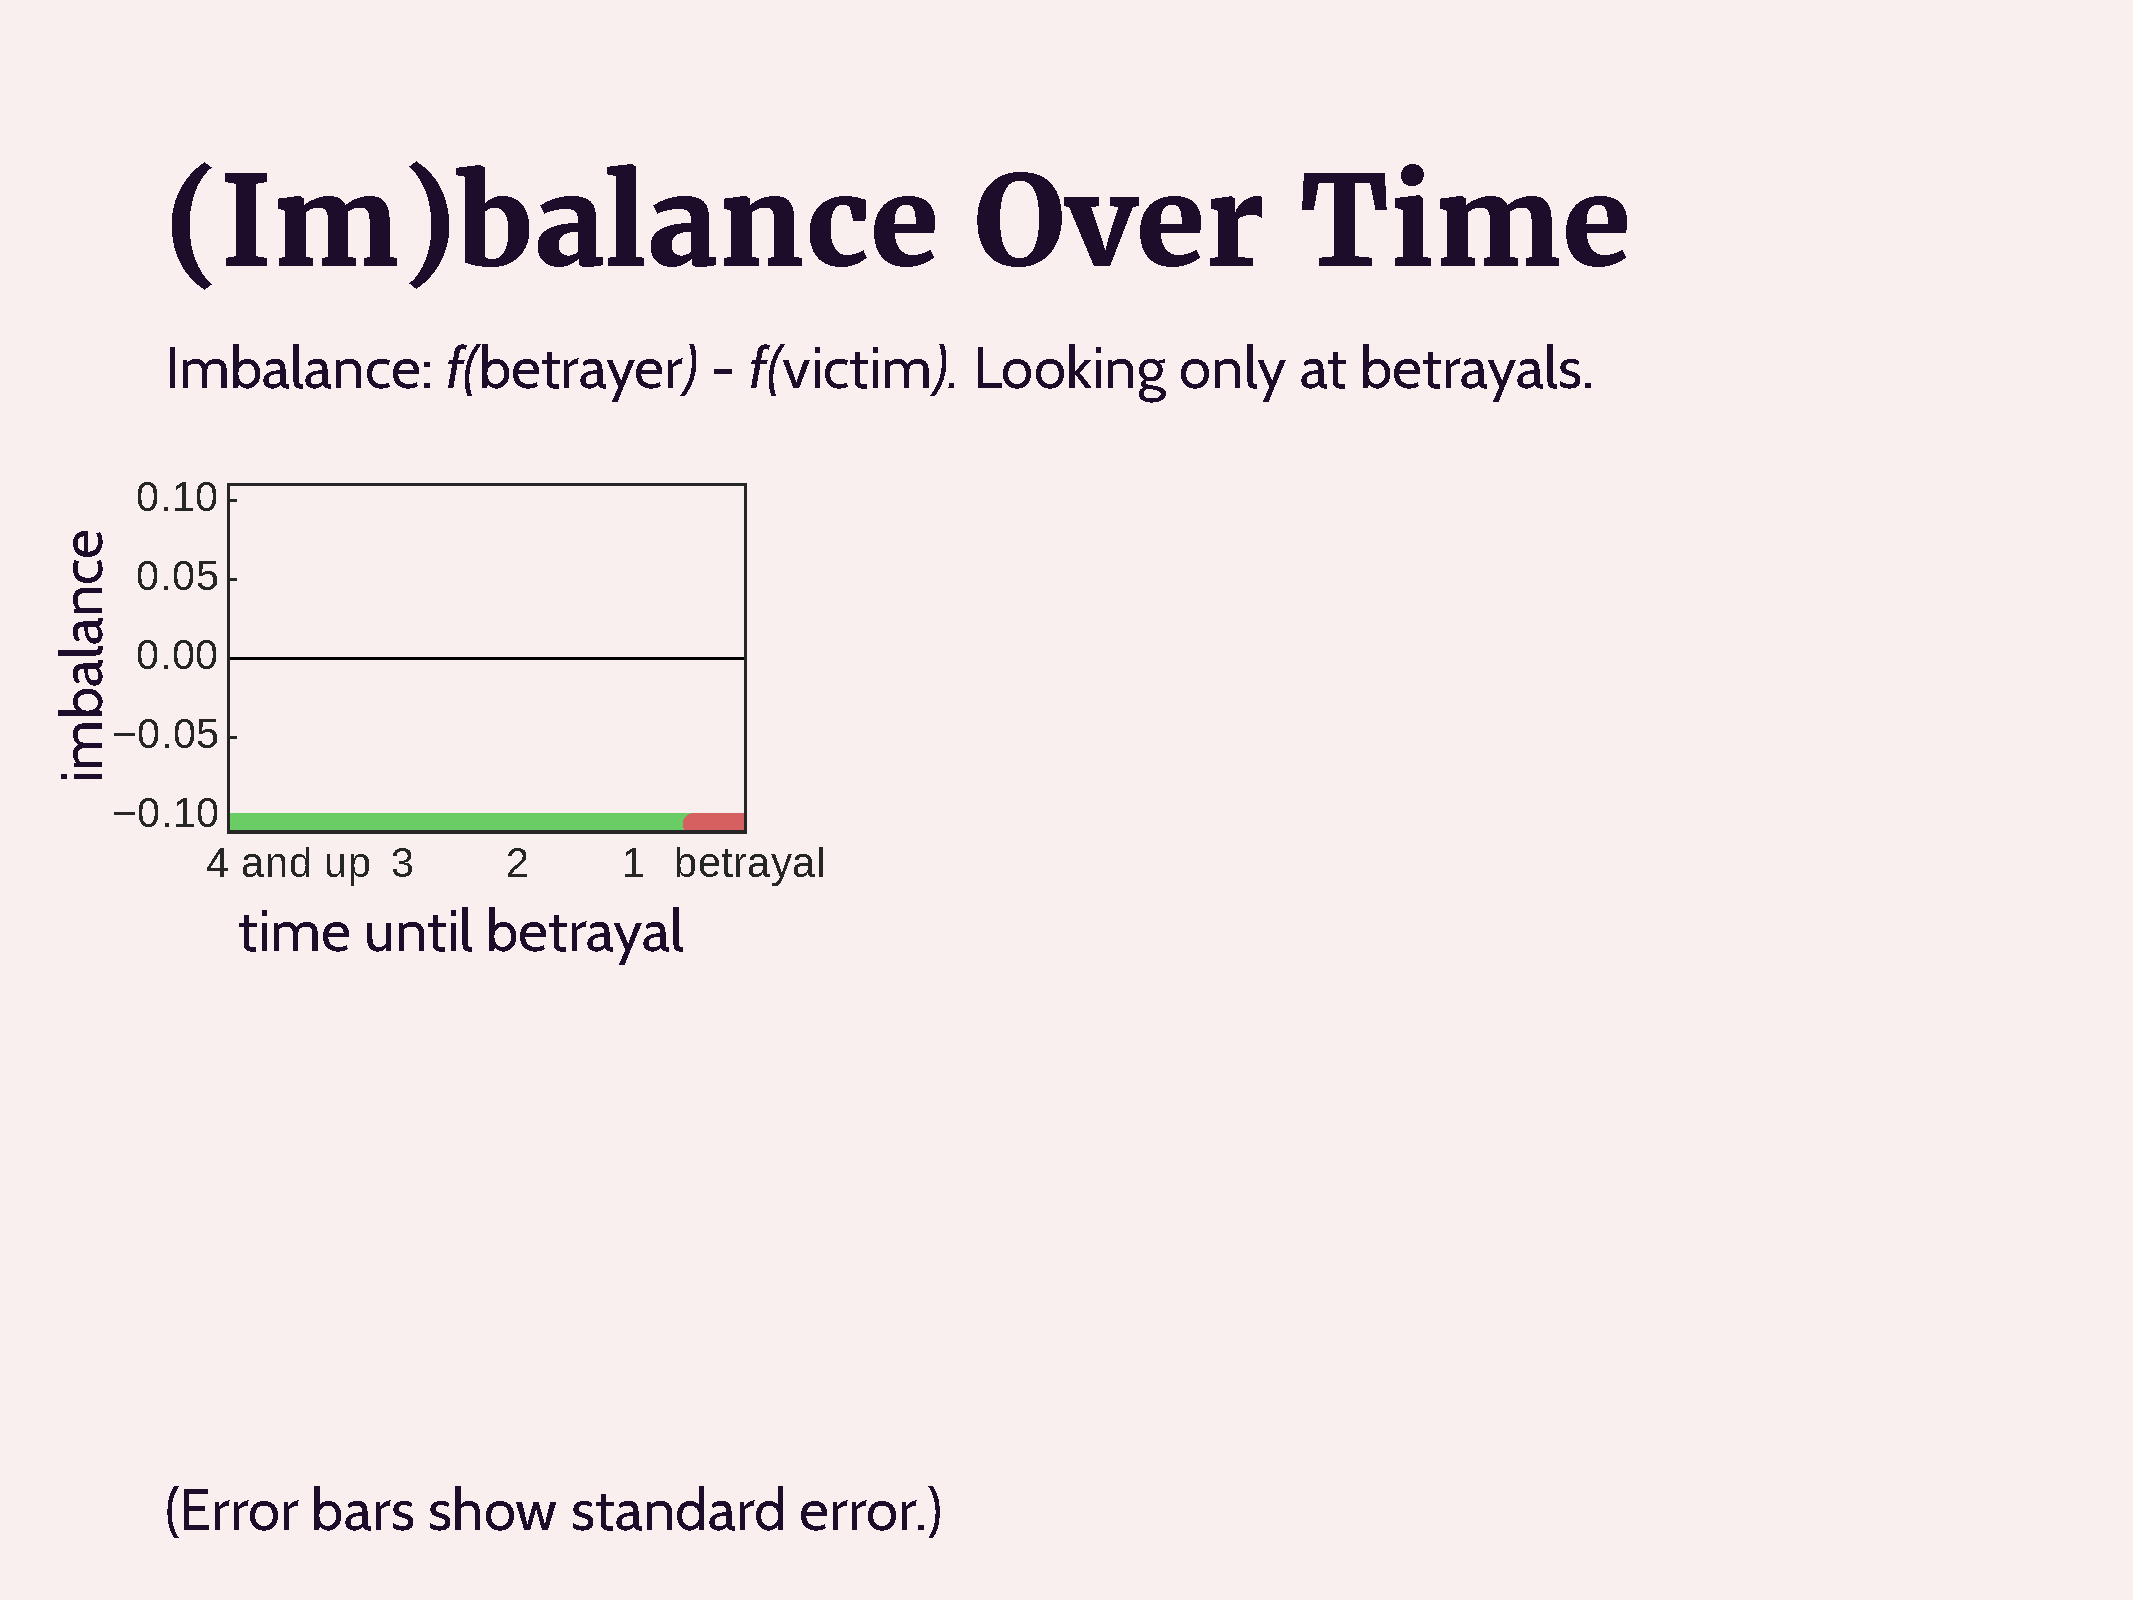
\includegraphics[page=1,width=\paperwidth]{diplomacy/betrayal-results}}}
\only<2>{\makebox[\linewidth]{\includegraphics[page=2,width=\paperwidth]{diplomacy/betrayal-results}}}
\only<3>{\makebox[\linewidth]{\includegraphics[page=3,width=\paperwidth]{diplomacy/betrayal-results}}}
\only<4>{\makebox[\linewidth]{\includegraphics[page=4,width=\paperwidth]{diplomacy/betrayal-results}}}
\only<5>{\makebox[\linewidth]{\includegraphics[page=5,width=\paperwidth]{diplomacy/betrayal-results}}}
\only<6>{\makebox[\linewidth]{\includegraphics[page=6,width=\paperwidth]{diplomacy/betrayal-results}}}
\only<7>{\makebox[\linewidth]{\includegraphics[page=7,width=\paperwidth]{diplomacy/betrayal-results}}}
\only<8>{\makebox[\linewidth]{\includegraphics[page=8,width=\paperwidth]{diplomacy/betrayal-results}}}
\only<9>{\makebox[\linewidth]{\includegraphics[page=9,width=\paperwidth]{diplomacy/betrayal-results}}}
\only<10>{\makebox[\linewidth]{\includegraphics[page=10,width=\paperwidth]{diplomacy/betrayal-results}}}
\only<11>{\makebox[\linewidth]{\includegraphics[page=11,width=\paperwidth]{diplomacy/betrayal-results}}}

\end{frame}


\begin{frame}{But attack is only a proxy\dots}

  \begin{columns}
    \column{.35\linewidth}
  \begin{itemize}
  \item We really care about lies!
  \item Create new platform
  \item After sending every message
    \begin{itemize}
    \item Did they lie
    \item Did the person who sent them a message lie?
    \end{itemize}
  \end{itemize}
  \column{.65\linewidth}
    \gfxd{interface}{.9}
 \end{columns}
\end{frame}

\begin{frame}{Ontology of Lies}
  \footnotesize
\begin{tabularx}{\textwidth}{r  l |  X X}
	
& &\multicolumn{2}{l}{\textbf{Victim Reception}} \\

& &  \textbf{Trusting}&  \textbf{Suspicious} \\
\toprule
\multirow{2}{*}{ \rotatebox[origin=r]{90}{\textbf{Betrayer Veracity}}} & \textbf{Honest}
& \alert<2>{\textbf{Straightforward}}
\only<2->{Salut! Just checking in, letting you know the embassy is open, and if you decide to move in a direction I might be able to get involved in, we can probably come to a reasonable arrangement on cooperation.  Bonne journee!}
& \alert<5>{\textbf{Cassandra}}
\only<5->{I don't care if we target T first or A first. I'll let you decide. But I want to work as your partner. \dots I literally will not message anyone else until you and I have a plan. I want it to be clear to you that you're the ally I want.}
\\
& \textbf{Deception}
& \alert<4>{\textbf{Deceived}}
\only<4->{You, sir, are a terrific ally. This was more than you needed to do, but makes me feel like this is really a long term thing! Thank you.}
& \alert<3>{\textbf{Caught}}
\only<3->{So, is it worth us having a discussion this turn? I sincerely wanted to work something out with you last turn, but I took silence to be an ominous sign.}
\\

\end{tabularx}
\end{frame}


\begin{frame}{Skewed Distribution}

  \gfxd{Distribution}{.845}
  
\end{frame}


\begin{frame}{Evolution of a Game}

  \only<1>{\gfxd{game_lies_1}{.8}}
  \only<2>{\gfxd{game_lies_2}{.8}}
  \only<3>{\gfxd{game_lies_3}{.8}}
  \only<4>{\gfxd{game_lies_4}{.8}}
  \only<5>{\gfxd{game_lies_5}{.8}}
  \only<6>{\gfxd{game_lies_6}{.8}}
  \only<7>{\gfxd{game_lies_7}{.8}}
  \only<8>{\gfxd{game_lies_8}{.8}}
  \only<9>{\gfxd{game_lies_9}{.8}}
  \only<10>{\gfxd{game_lies_10}{.8}}
  \only<11>{\gfxd{game_lies_player}{.8}}
  \only<12>{\gfxd{game_lies_year}{.8}}
  \only<13>{\gfxd{game_lies_10}{.8}}
\end{frame}

\begin{frame}{Who can detect lies?}
\begin{center}
	\begin{tabular}{ l c }
		\toprule
		\textbf{}            & \textbf{MACRO F1}  \\ 
		\hline			
		\textbf{Predict all as Truth}       &0.47 \\ 
\pause
                \textbf{Predict all as  Lie}       & 0.11  \\
		\textbf{Random}      & 0.43	\\ 
\pause
                \textbf{Human}       & 0.55	\\ 
\pause
                \textbf{Neural-Word} &	0.52 \\ 
		\textbf{Neural-LSTM} &	0.50 \\ 
		\bottomrule
	\end{tabular}
\end{center}
\end{frame}

\begin{frame}{Excuses}

  \begin{itemize}
    \item Yeah, i actually botched my move because i forgot to click submit in the browser :/. Not that it would have made a difference. Hope you’re enjoying Belgium.
Okay, I’m so sorry. I got distracted again. Will you allow me a build this turn or do you plan on retaking Greece now?
    \item Hi Turkey! I’m sorry that I’ve been so slow to get in touch. Kind of a rough day for me to begin a game as I e been pretty swamped. Things are clearing up now, and I appreciate you reaching out to me.
              \item That was less a lie, and more my having changed my plans to be in line with what I messaged you, but not being able to update my orders in time.
  \end{itemize}
  
\end{frame}

\begin{frame}{Building Trust}

  \begin{itemize*}
    \item So tell me, how do you find Terraforming Mars? I'm a bit of a highkey space fanatic and one of my friends has been on me to try it forever, but I don't find I have a lot of time for gaming. Worth a look? Or something that's fun but not for long?
        \item \alert<2>{Maine is beautiful! I used to go to scout camp there.}
    \item To be honest, just got done with a day from hell, so not really thinking big picture at the moment yet. Placeholder orders are more or less just a standard French opening, just starting to touch base with all the neighbors.
  \end{itemize*}

\end{frame}

% \begin{frame}{Come to UMD}

% \begin{columns}
% 	\column{.5\linewidth}
%         \only<1>{
%         	\begin{center}
% 		
\includegraphics[width=.9\linewidth]{umd/umd} \\
% 		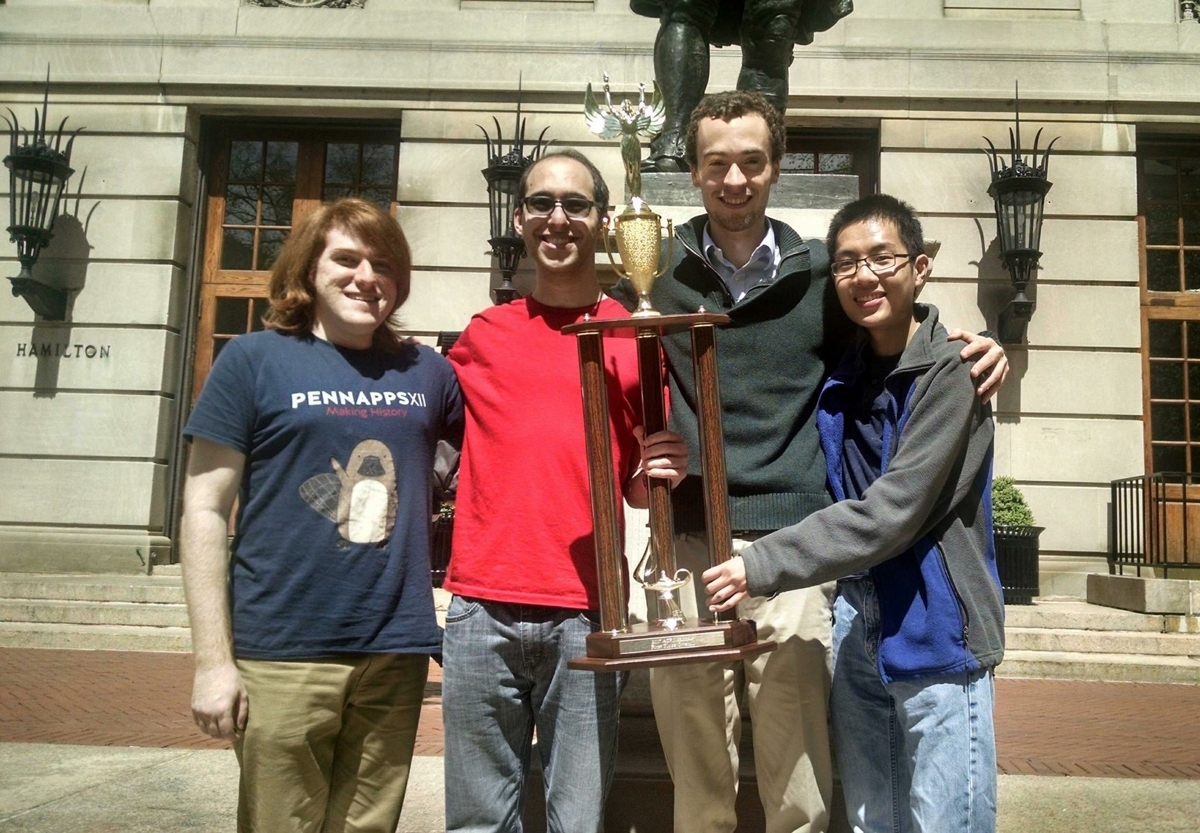
\includegraphics[width=.9\linewidth]{umd/qb_team}
% 	\end{center}
%               }
% 	\column{.5\linewidth}
% 		\begin{itemize}
%                 \item Looking for undergrads/grads/interns
%                 \item A great place for natural language
%                   processing and machine learning
%                 \item Not too shabby at quiz bowl either
% 		\end{itemize}
% \end{columns}

% \end{frame}

\begin{frame}{Future Steps}

  \begin{itemize}
    \item Sequence-dependent predictions
    \item Interactive predictions to help victims detect lies
    \item Scaling up data collection
  \end{itemize}
\end{frame}


\begin{frame}{Collecting Tricky Text}

  \begin{itemize}
    \item Engage with motivated, expert communities
    \item Make the task fun
    \item Align users' fun with research interests
    \item Show them what you're doing, get them involved
  \end{itemize}

\end{frame}


\frame{
  \frametitle{But wait, there's more!}

  \vspace{-.5cm}

\begin{columns}



  \column{.5\linewidth}


    \begin{block}{\sout{Buy} Read my book!}
      \begin{center}
        
\includegraphics[width=0.3\linewidth]{general_figures/applications_of_tm}
      \cite{boyd-graber-17}
       \end{center}
    \vspace{-.3cm}
    \end{block}


    \begin{block}{Interactive Machine Learning}
     \centering
        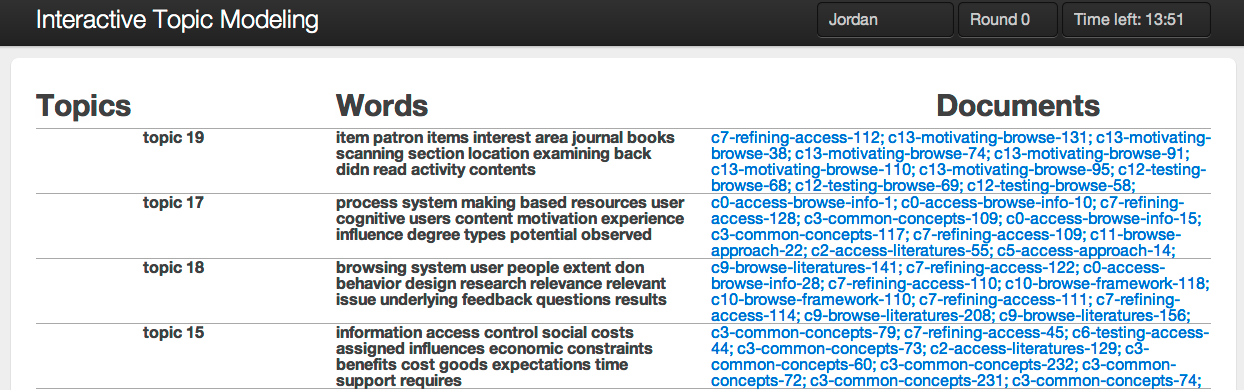
\includegraphics[width=0.4\linewidth]{interactive_topic_models/new_interface} \\
       \cite{Smith-17,Poursabzi-16}
    \end{block}



  \column{.5\linewidth}

   \begin{block}{Computational Political Science}
     \centering
     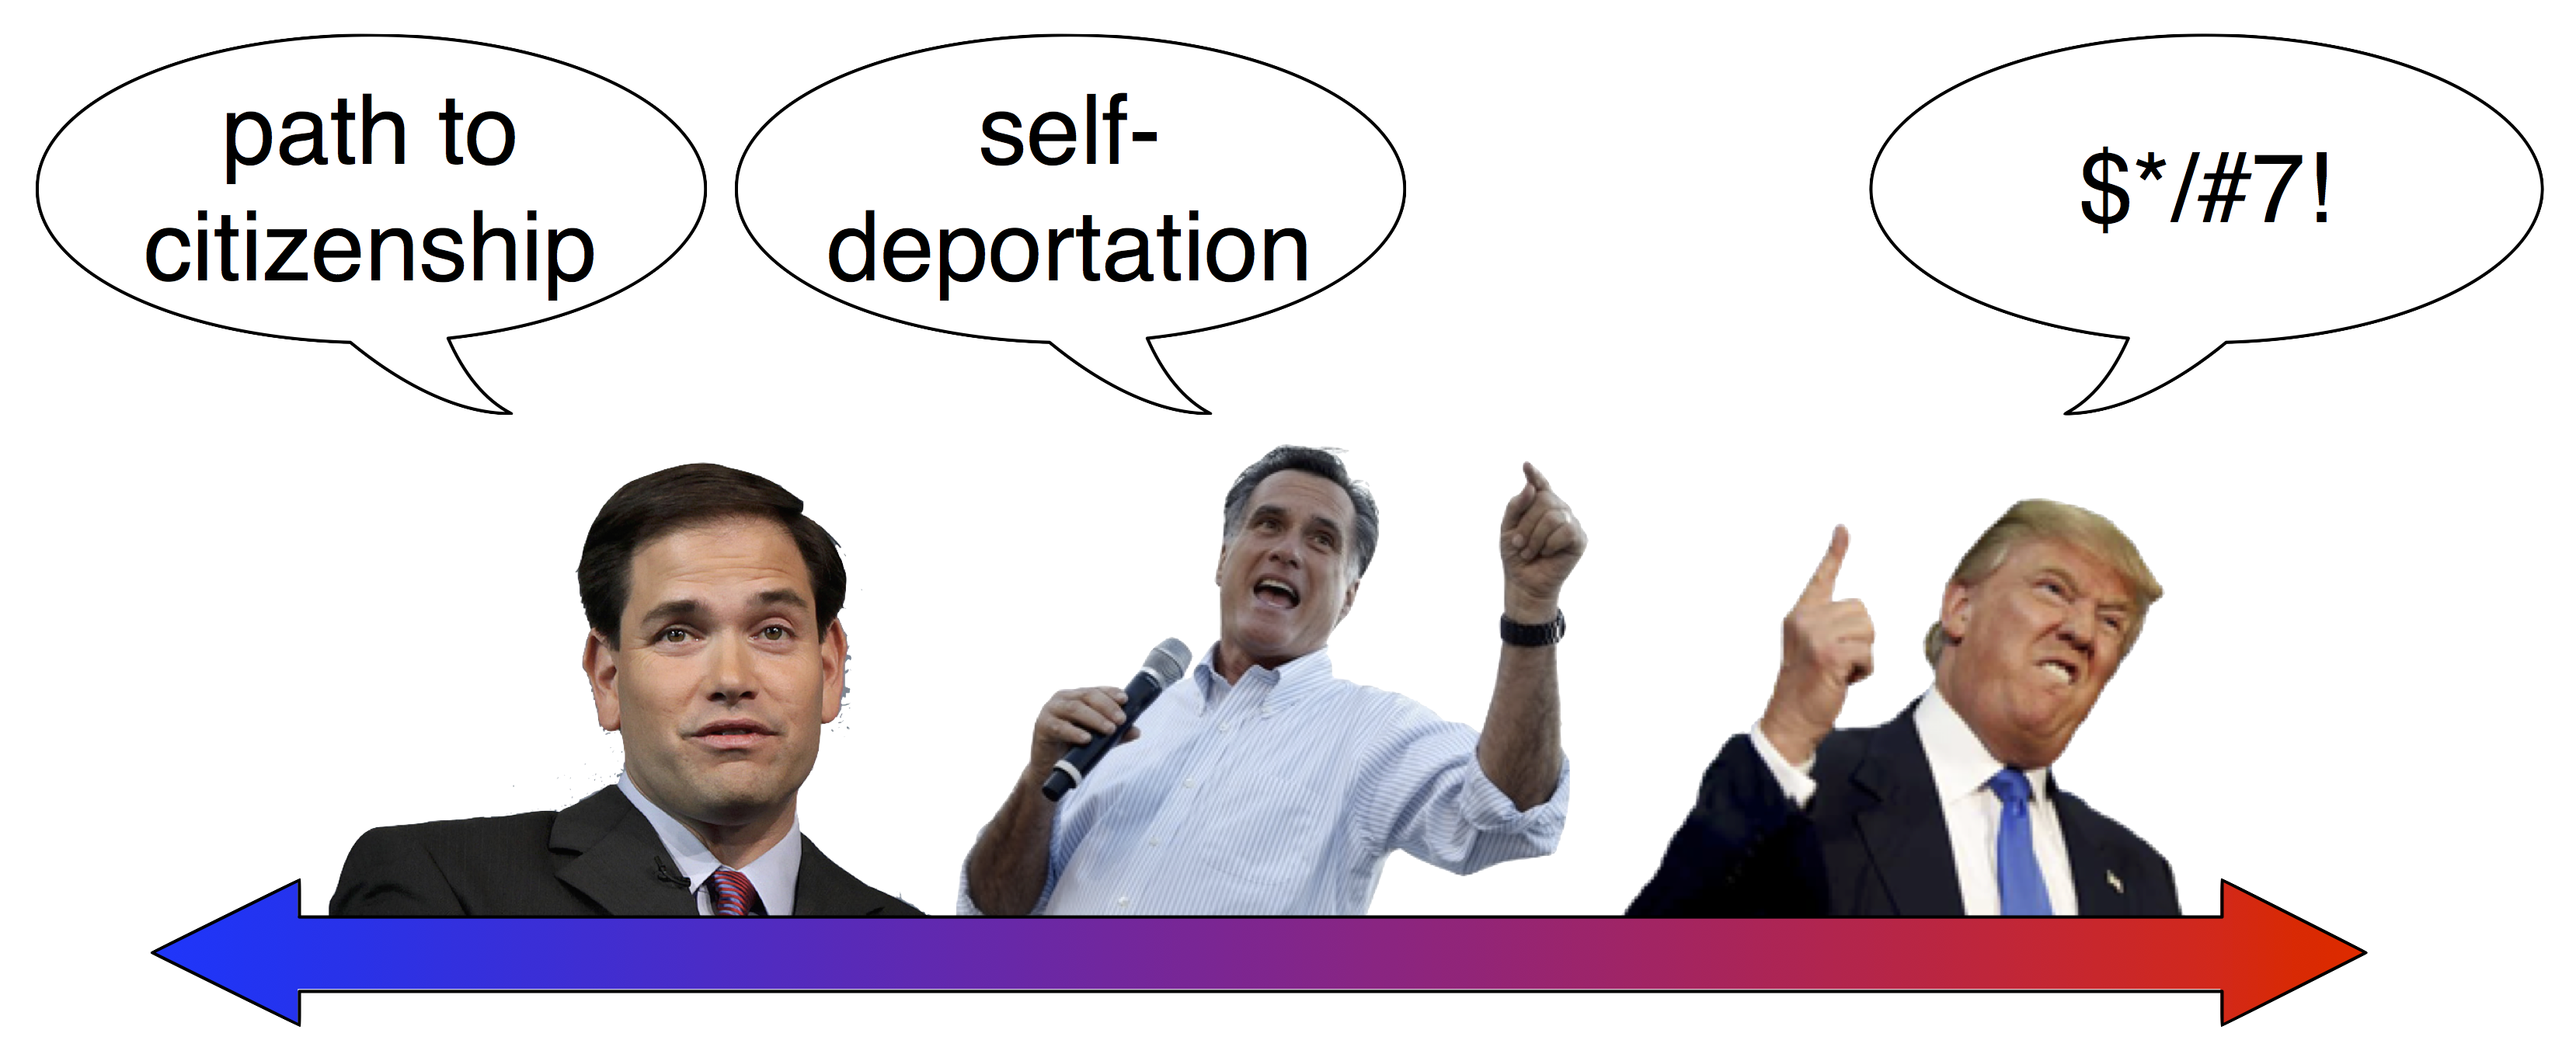
\includegraphics[width=0.8\linewidth]{teaparty/figures/framing} \\
     \cite{nguyen-13b,nguyen-15}
   \end{block}



    \begin{block}{Computer Vision}
    \centering
        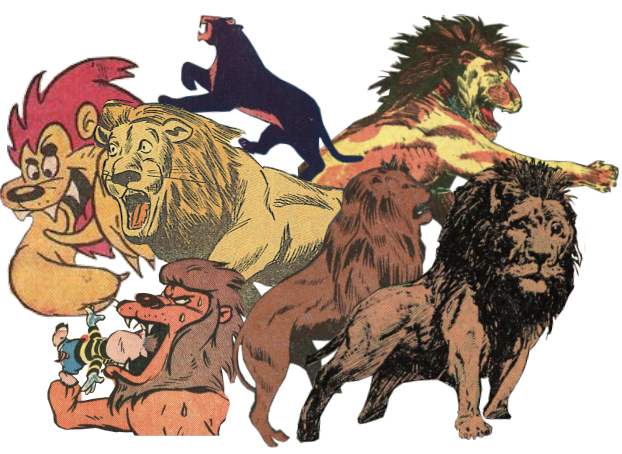
\includegraphics[width=0.5\linewidth]{general_figures/comics} \\
        \cite{Hu-12b,iyyer-17}
    \end{block}



\end{columns}

}




\frame{

	\frametitle{Thanks}

        \begin{block}{Collaborators (not listed on previous slides)}
          Anupam Guha (Maryland), Manjhunath Ravi (Colorado), Danny Bouman (UMD UG),
          Stephanie Hwa (UMD UG), Yogarshi Vyas (UMD), Larry Davis
          (UMD), Naho Orita (Tohoku), Snigdha Chaturvedi (UMD), Varun
          Manjunatha (UMD), Srijan Kumar (UMD), Vlad Niculae
          (Cornell), Cristian Danescu-Niculescu-Mizil (Cornell),
          Richard Socher (Salesforce), Leonardo Claudino (UMD)
        \end{block}

	\begin{columns}

	\column{.5\linewidth}
        \begin{block}{Funders}
        \begin{center}
          
\includegraphics[width=0.4\linewidth]{general_figures/nsf}
       \end{center}
        \end{block}

	\column{.5\linewidth}
        \begin{block}{Supporters}
        	\gfxq{naqt}{.4}
        \end{block}

        \end{columns}
}

\begin{frame}[plain]

\begin{columns}
  \column{.3\linewidth}
        \begin{center}
          @boydgraber
          
\includegraphics[width=0.6\linewidth]{general_figures/twitter}
          \\
          \end{center}
  \column{.65\linewidth}

  \begin{center}
    https://www.youtube.com/c/JordanBoydGraber
    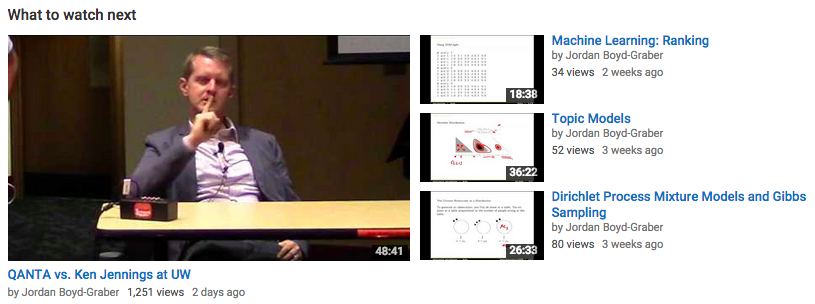
\includegraphics[width=1.0\linewidth]{general_figures/youtube} \\

\end{center}

\end{columns}

\begin{center}
\huge
http://qanta.org \\
http://boydgraber.org
       \end{center}


\end{frame}

\begin{frame}{References}
\bibliographystyle{style/acl}
\tiny
\bibliography{bib/journal-full,bib/jbg}
\end{frame}


\begin{frame}{Who can detect lies?}
	\begin{tabular}{ l l l l l }
		\toprule
		\textbf{}            & \textbf{Lie F1}        & \textbf{Truth F1} & \textbf{MACRO F1} & \textbf{MICRO F1}      \\ 
		\hline			
		\textbf{Predict all as Truth}       &0	& 0.937 &	0.469 &	0.882\\ 
\pause
                \textbf{Predict all as  Lie}       & 0.212	& 0	& 0.106 & 	0.119 \\
		\textbf{Random}      & 0.202	& 0.649	& 0.426	& 0.513\\ 
\pause
                \textbf{Human}       & 0.207	& 0.892	& 0.549	& 0.801	\\ 
\pause
                \textbf{Neural-Word} &       0.24 &	0.802 &	0.521 &	0.686  \\ 
		\textbf{Neural-LSTM} &        0.126 &	0.871 &	0.498 &	0.776 \\ 
		\bottomrule
	\end{tabular}
\end{frame}


\begin{frame}{Our QA Systems are Crazy}

\only<1-2>{
\begin{block}{Out of Touch}
On ``The Critic'', this man was replaced by a drunken animatronic bear from the Country Bear Jamboree but nobody seemed to notice.  This man was edited to appear in the film "Contact", which prompted an angry statement from Mike McCurry.  He was portrayed by Dennis Quaid in "The Special Relationship", who ate McDonald's every day to prepare for the role.  A fictionalized version of this man named Henry Burton, a charismatic Southern governor running for the Democratic nomination, is portrayed by John Travolta in "Primary Colors".  For ten points, name this American president who played the saxophone on an appearance on the Arsenio Hall Show.
\end{block} }
\only<2>{{\bf Samuel L. Jackson?}}

\end{frame}


\begin{frame}{Matching Entites Across Sentences}

\begin{block}{\only<2->{Magic Flute}}

    At its premiere, \alert<3>{the librettist of this opera} portrayed
    \alert<4>{a character who asks for a glass of wine with his dying wish}. \alert<4>{That
    character} in this opera is instructed to ring some bells to summon
    his love. At its beginning, \alert<5>{a man} who claims to have killed a (*)
    serpent has a padlock put on \alert<5>{his} mouth because of \alert<5>{his} lying. The
    plot of this opera concerns a series of tests that \alert<5>{Tamino} must
    undergo to rescue Tamina from Sorastro. For 10 points, name this
    Wolfgang Mozart opera titled for \alert<6>{an enchanted woodwind instrument}.
\end{block}



\only<3-4>{{\bf Not all references are named (\alert<3>{Emanuel
      Schikaneder}, \alert<4>{Papageno})}}
\only<5>{Need to be able to match pronouns across sentences (or have
  deep world knowledge)}
\only<6>{Requires semantic knowledge}
\end{frame}



\begin{frame}{How can this fail?}

  \only<1>{\gfxq{opponent_fail1}{.8}}
  \only<2>{\gfxq{opponent_fail2}{.8}}
  \only<3>{\gfxq{opponent_fail3}{.8}}
  \only<4>{\gfxq{opponent_fail4}{.8}}
  \only<5>{\gfxq{opponent_fail5}{.8}}
  \only<6>{\gfxq{opponent_fail6}{.8}}
  \only<7>{\gfxq{opponent_fail7}{.8}}

\end{frame}

\begin{frame}{Can we do better?}

  \only<1>{\gfxq{dqn_overview2}{.8}}
  \only<2>{\gfxq{dqn_overview3}{.8}}
  \only<3>{\gfxq{dqn_overview4}{.8}}

\end{frame}


\begin{frame}{Comparing Models}

  \begin{itemize}
    \item Single-Player
    \item Deep Q-Network (DQN): World=Opponent~\cite{mnih-15}
      \begin{itemize}
        \item Learn representation of state to estimate $Q$-function
        \item Generalization of regression-based methods
        \item Similar to our representation of content
      \end{itemize}
    \item Deep Reinforcement Opponent Network (DRON)
  \end{itemize}

\end{frame}


\begin{frame}[plain]


\only<4->{\vspace{-.5cm}}

  \begin{columns}[T]
    \column{.3\linewidth}

    \only<1->{ 
\includegraphics[width=2\linewidth]{qb/feature_ex_l_1} \\ }
    \vspace{.5cm}
    \only<4->{ \includegraphics[width=2\linewidth]{qb/feature_ex_l_2}  \\ }
    \vspace{.5cm}
    \only<7->{ \includegraphics[width=2\linewidth]{qb/feature_ex_l_3}  \\ }


    \column{.68\linewidth}
    \vspace{-.5cm}
    \only<2->{ \includegraphics[width=.85\linewidth]{qb/feature_ex_r_1} \\ }
    \only<3->{ \vspace{-.5cm} \hspace{.5cm} \includegraphics[width=.1\linewidth]{qb/feature_ex_wait}  \\ }
    \only<5->{ \includegraphics[width=\linewidth]{qb/feature_ex_r_2} \\ }
    \only<6->{ \vspace{-.5cm} \hspace{.5cm}\includegraphics[width=.1\linewidth]{qb/feature_ex_wait}  \\ }
    \only<8->{ \includegraphics[width=\linewidth]{qb/feature_ex_r_3} \\ }
    \only<9->{ \vspace{-.5cm} \hspace{.5cm} \includegraphics[width=.1\linewidth]{qb/feature_ex_buzz}  \\ }
    \only<9->{Answer: {\bf Julius Caesar}}
  \end{columns}

\end{frame}


\begin{frame}{Add more features: DRON-concat}

  \gfxq{dron-concat}{.8}

\end{frame}


\begin{frame}{Error Analysis}

  \only<1>{\gfxq{error1}{.8}}
  \only<2>{\gfxq{error2}{.8}}
  \only<3>{\gfxq{error3}{.8}}
  \only<4>{\gfxq{error4}{.8}}
  \only<5>{\gfxq{error5}{.8}}
  \only<6>{\gfxq{error6}{.8}}
  \only<7>{\gfxq{error7}{.8}}

\end{frame}



\begin{frame}{How the shared task works}

\begin{columns}
  \column{.3\linewidth}
  \gfxq{bamber}{.5}

  \column{.65\linewidth}
  \begin{itemize}
    \item<3-> Hi! Available questions are \texttt{[1,2,3,4]}
    \item<5-> It's \texttt{Extremism}
    \item<7-> It's \texttt{in}
    \item<9-> It's \texttt{the}
    \item<11-> Got it!  You've answered Question 1 at Position
      3 with \texttt{Barry\_Goldwater}
  \end{itemize}

\end{columns}


\begin{columns}

  \column{.65\linewidth}
  \begin{itemize}
    \item<2-> I'm User~1.  I’d like to play!
    \item<4-> I’d like to hear Word~1 of Question 1
    \item<6-> I’d like to hear Word~2 of Question 1
    \item<8-> I’d like to hear Word~3 of Question 1
    \item<10-> I’d like to answer Question 1 with
      \texttt{Barry\_Goldwater}
    \end{itemize}
  \column{.3\linewidth}
  \only<2->{\gfxq{buzzer}{.5}}
\end{columns}

\end{frame}


\begin{frame}{Where we have problems}

\only<1-2>{
\begin{block}{Out of Date}
Although he won the California primary in 2000, he distanced himself
from fellow reform presidential candidate Pat Buchanan by comparing
him to Attila the Hun. After being called a jackass, he prompted
Lindsey Graham to destroy his phone by giving out his number during a
speech. The slogan (*) Make America Great Again has been used by this
politician, who claimed he didn't like people who were captured as a
slight to John McCain and kicked off his 2016 presidential bid with
some inflammatory remarks about Mexicans. For 10 points, name this
Republican candidate and real estate mogul.
\end{block} }
\only<2>{{\bf Chris Christie?}}

\only<3-4>{
\begin{block}{Out of Touch}
  This singer recently cancelled the Great Escape Tour, and, in one
  song, she claims that she will be ``Eating crumpets with the sailors
  / On acres without the neighbors.'' She collaborated with Jennifer
  (*) Hudson on the song ``Trouble,'' which was issued in her album
  update Reclassified. This artist of ``Change Your Life'' was
  inspired by scenes from the movie Clueless to make the music video
  for a song in which she collaborated with Charli XCX. For 10 points,
  name this Australian rapper whose album The New Classic contained
  ``Fancy.''
\end{block} }
\only<4>{{\bf Bruce Springsteen?}}

\end{frame}



\end{document}
